\chapter{Introduction}

This book is grew out from a course that 
Masaki Kashiwara gave at the ``Universit\'e Paris-Nord'' 
during the first term of the academic year 1976--77. 
Teresa Monterio Fernandes worked out lecture notes for 
this course, which were preprinted in 1979 by Paris-Nord 
under the title ``Syst\`ems d'\'equations 
microdiff\'erentielles'' and distributed to a happy few. 
On the grounds that such a basic textbook 
should be made available to a wider mathematical audience, 
the Birkh\"auser Publishing Company proposed to make it 
a new volume of its series ``Progress in Mathematics''. 
Kashiwara and the publisher agreed not to change the overall 
structure of the text (which at first 
was supposed to be provisional); T. Monterio Fernandes then 
was kind enough to make care of the translation into English 
and of the necessary minor corrections. 

It was decided that an introduction might be written, outlining 
the purposes and main features of the text, and mentioning 
recent developments connected with the index fomula in Chapter \ref{ch6}. 
Kashiwara suggested that I would write this introduction, 
and I accepted to do so with pleasure. 
I thought it might be a way of thanking Kashiwara for 
all he has taught me since I benefited so much from 
talking to him and reading his works. 

In short, this book is an introduction to systems of 
microdifferential equations and to some of the tools 
of micro-local analysis. 
Here a remark on the terminology; after \cite{BK76}, 
pseudo-differential operators on a complex manifold \(X\) 
were considered in \cite{SKK}: 
They used the notation \(\cP_X\) for the sheaf of rings 
of pseudo-differential operators (this was a sheaf on the 
projectivised cotangent bundles of \(X\)). 
In recent years, instead \(\cP_X\), 
one has been using \(\cE_X\) (now viewed as a sheaf of rings 
on the cotangent bundle itself); \(\cE_X\) is called 
the sheaf of \emph{micro-differential operators}: 
micro-differential operators are defined and studied 
locally in the cotangent bundle, i.e. \emph{microlocally}. 

As is well-known, say for \(X\) of complex dimension one 
with variable \(t\), 
both \(\frac{d}{dt}\) and \(
    \left(\frac{d}{dt}\right)^{-1}
\) are micro-differential operators (more precisely, 
as a section of \(\cE_X\), 
\(\left(\frac{d}{dt}\right)^{-1}\) is defined outside the
zero-section of the cotangent bundle). 
An infinite series \(
    \sum_{n\geqq0}^{}a_n(t)\left(\frac{d}{dt}\right)^{-n}
\) also defines a micro-differential operator, providing 
the holomorphic functions \(a_n(t)\) satisfy, 
on any compact \(K\) of \(X\), an estimate of the type 
\[
    \sup_{t\in K}\lvert a_n(t)\rvert < (n!)C_K^n,\quad\text{for~some \(C_K>0\).}
\]
There is no way to make such operators act on the space of 
holomorphic functions. However, 
let \(X=\cc\) and 
take a closed angular sector \(Z_\varepsilon\) inside 
the disk \(
    D_\varepsilon=\{t\in \cc; \lvert t\rvert <\varepsilon\}
\).
\begin{figure}[htb]
    \centering
    %\scalebox{0.8}{
        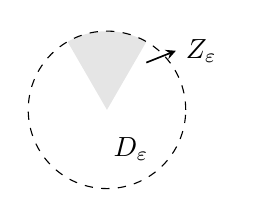
\begin{tikzpicture}[x=0.5cm,y=0.5cm]
        \fill[black!10] (1,1.73)arc(60:120:2)--(-1,1.73)-- (0,0)--cycle;
        \draw[dashed,black!100] (0.7,0.1) (0,0) ellipse (2 and 2);
        \draw[->,>=stealth,semithick] (1,1.2)--(1.75,1.5)node[right]{$Z_\varepsilon$}; %x軸
        \draw (1.3,-1) node[left]{$D_\varepsilon$};
    \end{tikzpicture}%}
    %\caption{開区間は円盤と閉区間の合併}
    %\label{fig:loc-closed-intersection}
\end{figure}\\%
Let \(\cO(D_\varepsilon)\) resp.~\(
    \cO(D_\varepsilon-Z_\varepsilon)
\) be the space of holomorphic functions on \(D_\varepsilon\) 
resp.~\(D_\varepsilon-Z_\varepsilon\); 
then \(\left(\frac{d}{dt}\right)^{-1}\) operates on \(
    \cO(D_\varepsilon-Z_\varepsilon)\mathbin{|}\cO(D_\varepsilon)
\), to get an operation of microdifferential operators,
it suffices to make \(\varepsilon\) smaller and smaller, i.e. 
to consider \(
    \indlim[\varepsilon\to0]
    \cO(D_\varepsilon-Z_\varepsilon)
    \mathbin{|}
    \cO(D_\varepsilon)
\).

The reader will find two definitions 

